\documentclass[10pt,a4paper,titlepage]{report}
\usepackage[utf8]{inputenc}
\usepackage{amsmath}
\usepackage{amsfonts}
\usepackage{amssymb}
\usepackage{graphicx}
\usepackage{xcolor}
\usepackage{minted}


\nonstopmode
\begin{document}
\begin{titlepage}
\author{Rwithik Manoj}
\title{Perl Scripts}
\date{\today}
\maketitle
\end{titlepage}

Create a text file and answer the following queries :
\begin{enumerate}
	\item Search for the pattern `apple’ in the file and display the number of occurences.
	\par
	\teftbf{Script: }\newline
	\inputminted[tabsize=4]{perl}{../Scripts/Perl/1a}
	\textbf{Output: }\newline
	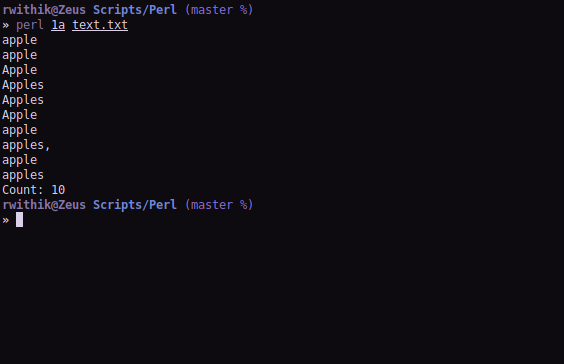
\includegraphics[width=\linewidth]{../Images/Perl/1a.png}
	\pagebreak
	\item Count the number of words that ends with `e’
	\par
	\teftbf{Script: }\newline
	\inputminted[tabsize=4]{perl}{../Scripts/Perl/1b}
	\textbf{Output: }\newline
	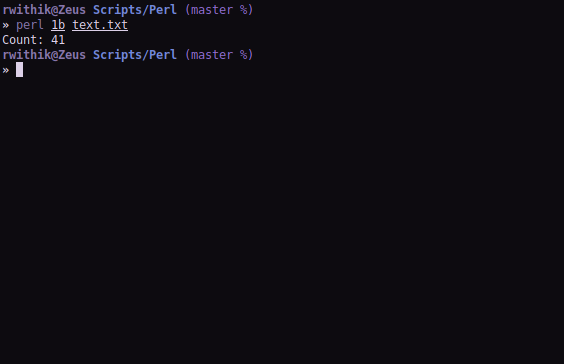
\includegraphics[width=\linewidth]{../Images/Perl/1b.png}
	\item Count the number of words that starts with `ap’
	\par
	\teftbf{Script: }\newline
	\inputminted[tabsize=4]{perl}{../Scripts/Perl/1c}
	\pagebreak
	\textbf{Output: }\newline
	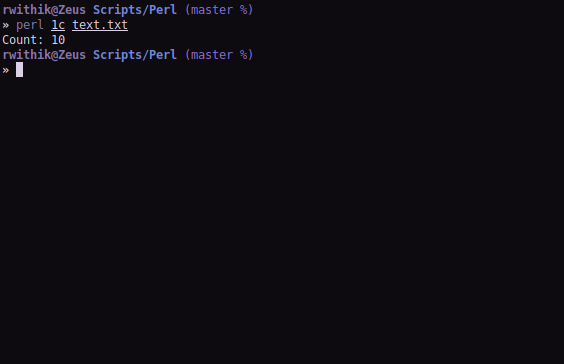
\includegraphics[width=\linewidth]{../Images/Perl/1c.png}
	\item Search for words containing `a’ or `s’
	\par
	\teftbf{Script: }\newline
	\inputminted[tabsize=4]{perl}{../Scripts/Perl/1d}
	\pagebreak
	\textbf{Output: }\newline
	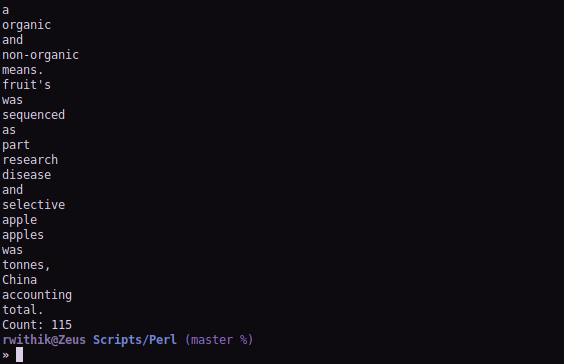
\includegraphics[width=\linewidth]{../Images/Perl/1d.png}
	\item Search for words containing zero or more occurrence of `e’
	\par
	\teftbf{Script: }\newline
	\inputminted[tabsize=4]{perl}{../Scripts/Perl/1e}
	\pagebreak
	\textbf{Output: }\newline
	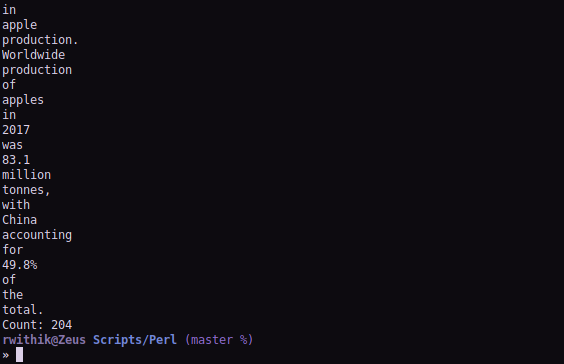
\includegraphics[width=\linewidth]{../Images/Perl/1e.png}
	\item Search for words containing one or more occurrence of `e’
	\par
	\teftbf{Script: }\newline
	\inputminted[tabsize=4]{perl}{../Scripts/Perl/1f}
	\pagebreak
	\textbf{Output: }\newline
	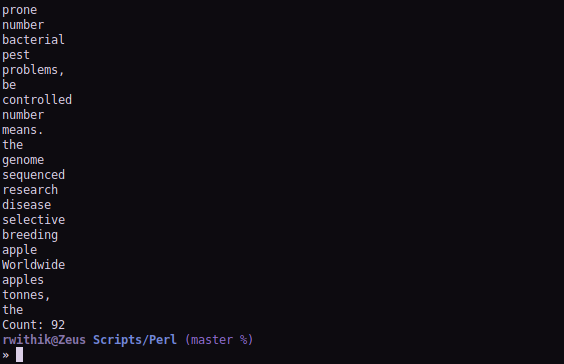
\includegraphics[width=\linewidth]{../Images/Perl/1f.png}
	\item Search for words containing the letters `l’ and `m’, with any number of characters in
	between
	\par
	\teftbf{Script: }\newline
	\inputminted[tabsize=4]{perl}{../Scripts/Perl/1g}
	\pagebreak
	\textbf{Output: }\newline
	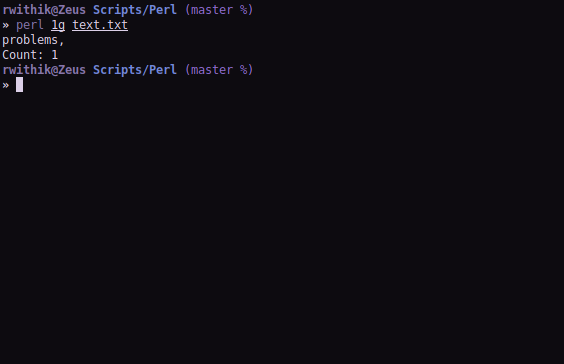
\includegraphics[width=\linewidth]{../Images/Perl/1g.png}
\end{enumerate}
\pagebreak
\par The text file used in the above screenshots:\newline\newline
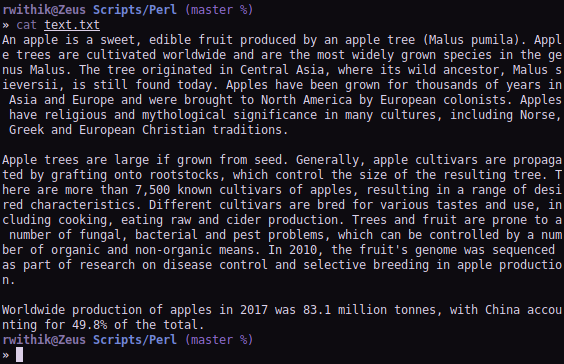
\includegraphics[width=\linewidth]{../Images/Perl/perl_text.png}

\end{document}
